\chapter{Algorithms and Implementation}

\section{Interface Implementation}\label{interface-implementation}

One of the core components of Foldlings is the interface. To create
features, we capture touch input, display a preview of the fold feature
as the user creates it, and add created features to the fold pattern.
This system is outlined in Figure \ref{mvc}.

\begin{figure}[htbp]
\centering
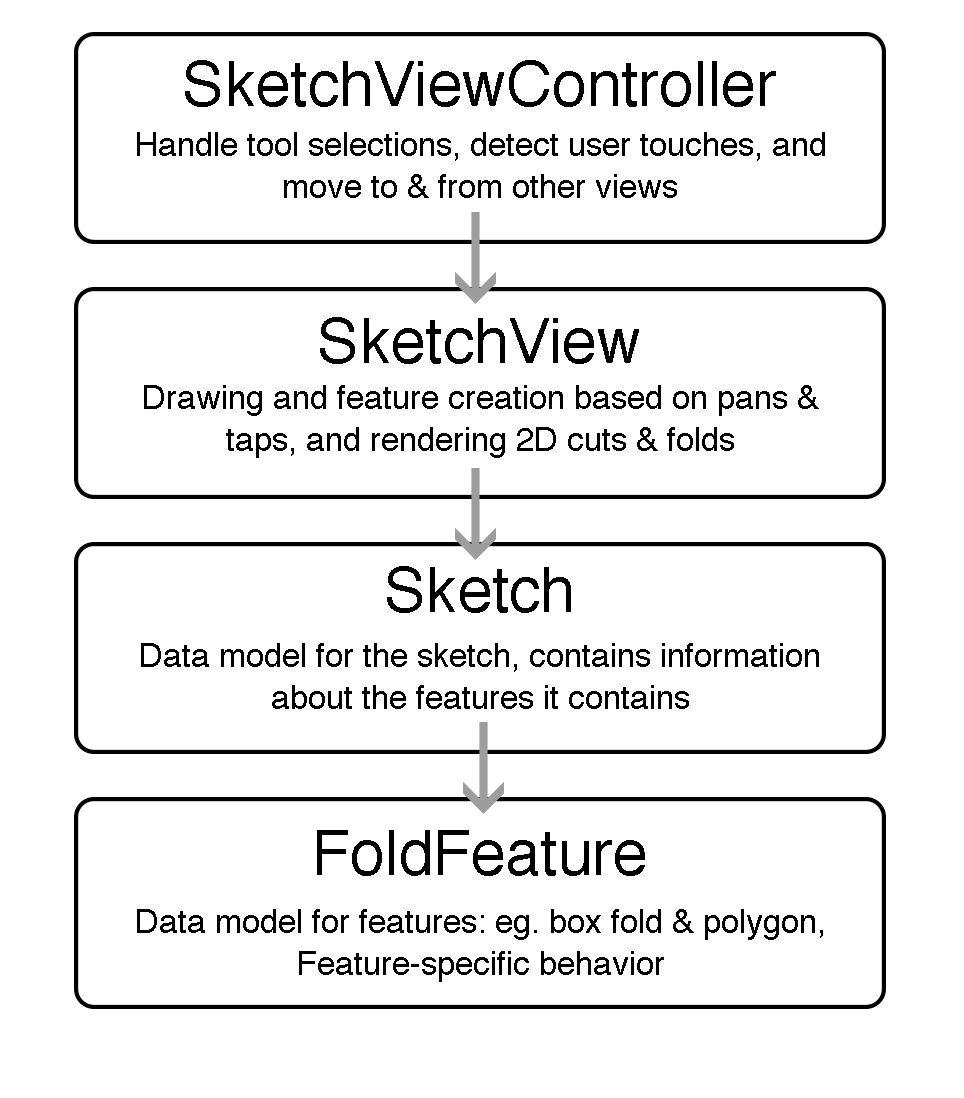
\includegraphics{figures/40_Tech_Interface_Implementation/sketchview-descendents-thesis-figure.png}
\caption{Relationship between interface classes: a SketchViewController
manages a SketchView that contains a Sketch that contains FoldFeatures.
\label{mvc}}
\end{figure}

Although this structure borrows heavily from the Model-View-Controller
design pattern, we do not follow the pattern strictly. The MVC paradigm
often becomes muddy, with much information shared between the separate
modules (\citet{veit2003model}). In our case, we separate modules not
purely based on MVC encapsulation but based on functionality. For
example, rather that strictly separating all touch handling into the
view controller or all drawing into the view, these responsibilities are
shared between the classes as needed to perform their roles. See section
\ref{touch-handling}, below, for more information.

\subsection{Touch Handling}\label{touch-handling}

In order to create features, we first need to capture touch input.
Foldings handles two types of touches: pan gestures, and tap gestures.
Apple describes gesture recognizers in the documentation for the
\emph{UIGestureRecognizer} class:

\begin{quote}
Gesture recognizers convert low-level event handling code into
higher-level actions. They are objects that you attach to a view, which
allows the view to respond to actions the way a control does. Gesture
recognizers interpret touches to determine whether they correspond to a
specific gesture, such as a swipe, pinch, or rotation. If they recognize
their assigned gesture, they send an action message to a target object.
The target object is typically the view's view controller, which
responds to the gesture\ldots{}
\end{quote}

In Foldlings, all gestures are captured by the SketchViewController,
which passes unhandled gesture on to classes lower down the chain. In
general, all taps are handled at the SketchViewController level; the
only exception to this rule is the Polygon feature, described in section
on page. \textbf{\textgreater{}\textgreater{}TODO PAGES}

\subsection{Tool Selection}\label{tool-selection}

Tool state is maintained by the SketchViewController. The
SketchViewController handles taps on tool buttons and features, and
passes pan gestures to the SketchView. The method called on the
SketchView depends on what feature was selected.

\small
\singlespacing 

\begin{pygmented}{swift}
    func handlePan(sender: AnyObject) {
        if(sketch.tappedFeature != nil){
            
            switch(sketch.tappedFeature!.activeOption!){
            case .MoveFolds:
                handleMoveFoldPan(sender)
            default: break
            }
        }
        else{
            switch (sketchMode) {
            case .BoxFold:
                handleBoxFoldPan(sender)
            case .FreeForm:
                handleFreeFormPan(sender)
            case .VFold:
                handleVFoldPan(sender)
            case .Polygon:
                handlePolygonPan(sender)
            default:
                break
            }
        }
    }
\end{pygmented}

\doublespacing
\normalsize

\textbf{\textgreater{}\textgreater{}TODO: CITE APPLE DOCS}

\subsection{Fold Feature Preview}\label{fold-feature-preview}

While the user is drawing, the SketchView displays a preview of the
feature in progress, to give feedback on the drawing. Meanwhile, the
SketchView also displays the previously drawn features that have been
added to the sketch. Although the display of cuts and folds for the
current feature is visually similar to those of the final feature, the
method of drawing a preview version of the feature varies from the
generation of final feature edges.

For polygons, we display

We store the separately, not added to the list of features.

We capture interpolation points a function of touch velocity. That is,
when the user draws more quickly, we capture more interpolation points
closer together. This allows us to capture the entire drawing with a
similar level of detail throughout, and correct for the gesture
recognizer sending relatively more frequent updates when the touch is
moving more slowly.

showing feature state

Drawing in progress Drawing features already in the sketch

\subsection{Feature Creation}\label{feature-creation}

Shading planes

Once the user completes a feature, we add it to the sketch\footnote{Assuming
  the feature is valid. \textbf{\textgreater{}\textgreater{}TODO: cite
  validity}}. The feature-specific implementations of the FoldFeature
superclass are described in Chapter \ref{tool-implementation} on page
\pageref{tool-implementation}. The Sketch class contains methods for
adding and removing features from the sketch. It also contains
lower-level functions for adding, removing, and replacing edges. These
methods are typically called by feature-specific methods that modify the
sketch.
